%*******************************************************************************
%*********************************** First Chapter *****************************
%*******************************************************************************

\chapter{Introduction}  %Title of the First Chapter
\graphicspath{{Chapter1/Figs/}}


Many biological processes can be transferred to well-studied models in statistical physics. Examples are ranging from the random walk model of mRNA during the transcription~\cite{Macdonald1968,Bressloff2013,Chou2011} to the evolution of ecological systems~\cite{Berryman1992,Butler2009,Sugihara2012,Williams2016a}. Analysis of these extracted models could help us to get useful insights into the corresponding biological problems. In this thesis, we are interested in modeling a molecular level biological problem, i.e. the motion of chromosomes in fission yeast during meiotic cell division~\cite{Chikashige1994,Vogel2009,Shibuya2014}.

Interestingly, during Prophase I of meiotic fission yeast, the nucleus containing three pairs of chromosomes move from one pole of the rod-like cell to the other, forming an oscillation behavior last for about two hours. The period of the oscillation is about $10$ minutes. Cells are divided into two after the oscillation is done~\cite{Yamamoto2001,Ding2004,Gerton2005}.

We are going to model this oscillation processes quantitatively with the chromosomes represented by polymer models~\cite{DeGennes1979,Doi1988}. The results we obtained from the modeling are used to explain relevant biological functionalities like chromosome alignment and gene recombinations~\cite{Lin2015}. 

In this chapter, we will introduce the biological backgrounds and some previous related studies about modeling chromosomes with polymers. We will propose our research goals and give an overview of the thesis in the last section. 


%********************************** %First Section  **************************************
\section{Nuclear oscillations in fission yeast} %Section - 1.2
\label{sec:nuclear_oscillations_in_fission_yeast}

In this section, we will introduce the biological basis of nuclear oscillation in fission yeast. We will firstly introduce our model organism, fission yeast. And then we show some basis of meiosis cell division. Next, we go into the nuclear structure of fission yeast and the movements of chromosomes, specifically during meiosis. The biological processes like chromosome alignment and recombination are discussed. In the last subsection, we discuss some understandings for the biological role of the nuclear oscillation.

\subsection{Fission yeast}
\label{sub:fission_yeast}

Fission yeast, also named \emph{Schizosaccharomyces pombe}, is a model organism that widely used in the study of molecular and cell biology. It is a unicellular eukaryote and has a rod-like shape. Typical size of fission yeast is $3$-$4$ micrometres in diameter and $7$-$14$ micrometres in length~\cite{Forsburg2003,Fantes2016}. See in Fig.~\ref{fig:fissionYeast} for a illustration of fission yeast.

\begin{figure}[htpb]
    \centering
    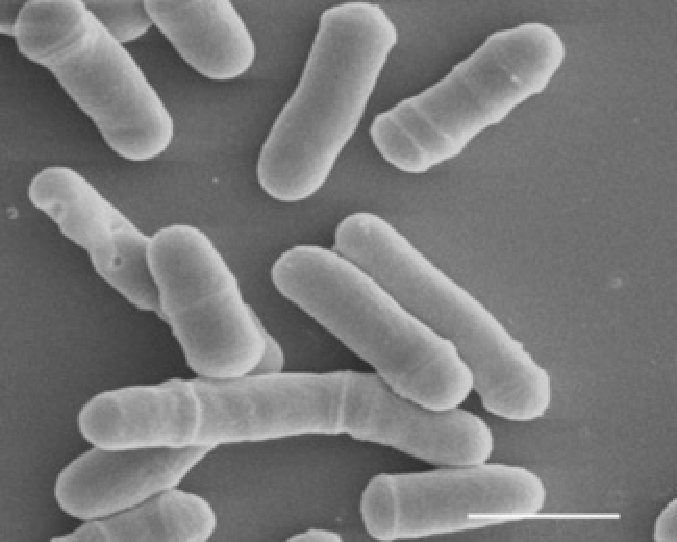
\includegraphics[width=0.5\linewidth]{fissionYeast}
    \caption{Microscopic view of a fission yeast culture. The scalar bar indicates $10$ $\mu$m. Image reprinted from~\cite{Morgan2007} with permission. }
    \label{fig:fissionYeast}
\end{figure}

Fission Yeast is widely used in traditional brewing and baking. It was first discovered in 1893 in the sediment of millet beer~\cite{Fantes2016,Hoffman2015}. As a single-celled fungus, fission yeast has a simple genome with three different chromosomes. The genome of fission yeast is fully sequenced and the three chromosomes contain about $14$Mb of DNA~\cite{Wood2002}. It has a rapid growth rate and easily manipulated to make mutants, which make it a perfect modeling organism for genetic studies. The growth of the fission yeast is simply by the elongation at the ends. After mitosis, division occurs by the formation a cell plate that cleaves the cell at its midpoint~\cite{Forsburg2003}. 

Fission yeast is normally a haploid cell. However, when put under stressful conditions, such as nitrogen deficiency, two cells will conjugate to form a diploid and then form four spores via meiosis~\cite{Coelho2013}. This is easy to observe experimentally and this stage is exactly when the interesting nuclear oscillation happens~\cite{Chikashige1994}. In the next subsection, we will explain the basis of the meiosis in fission yeast. 



\subsection{Basis of meiosis}
\label{sub:basis_of_meiosis}

Meiosis is a kind of cell division that reduces the number of chromosomes in the parent cell by half and produces four genetically distinct gamete cells. This process occurs in all the sexually reproducing organisms, including human~\cite{Freeman2008}. 

Meiosis begins with a parent cell with two copies of each chromosome, and is followed by two rounds of cell divisions which produce four potential daughter cells, each has half number of chromosomes as their parent cell. The two rounds of cell division are called \emph{Meiosis I} and \emph{Meiosis II}, respectively. It is during Meiosis I that the pair of chromosomes, one from the father and the other from the mother, separates into two offspring cells. Meiosis II is very similar to the mitosis where two sister chromatins separate~\cite{Freeman2008,Villeneuve2001a}. See an overview of meiosis in Fig.~\ref{fig:meiosis}.

\begin{figure}[htpb]
    \centering
    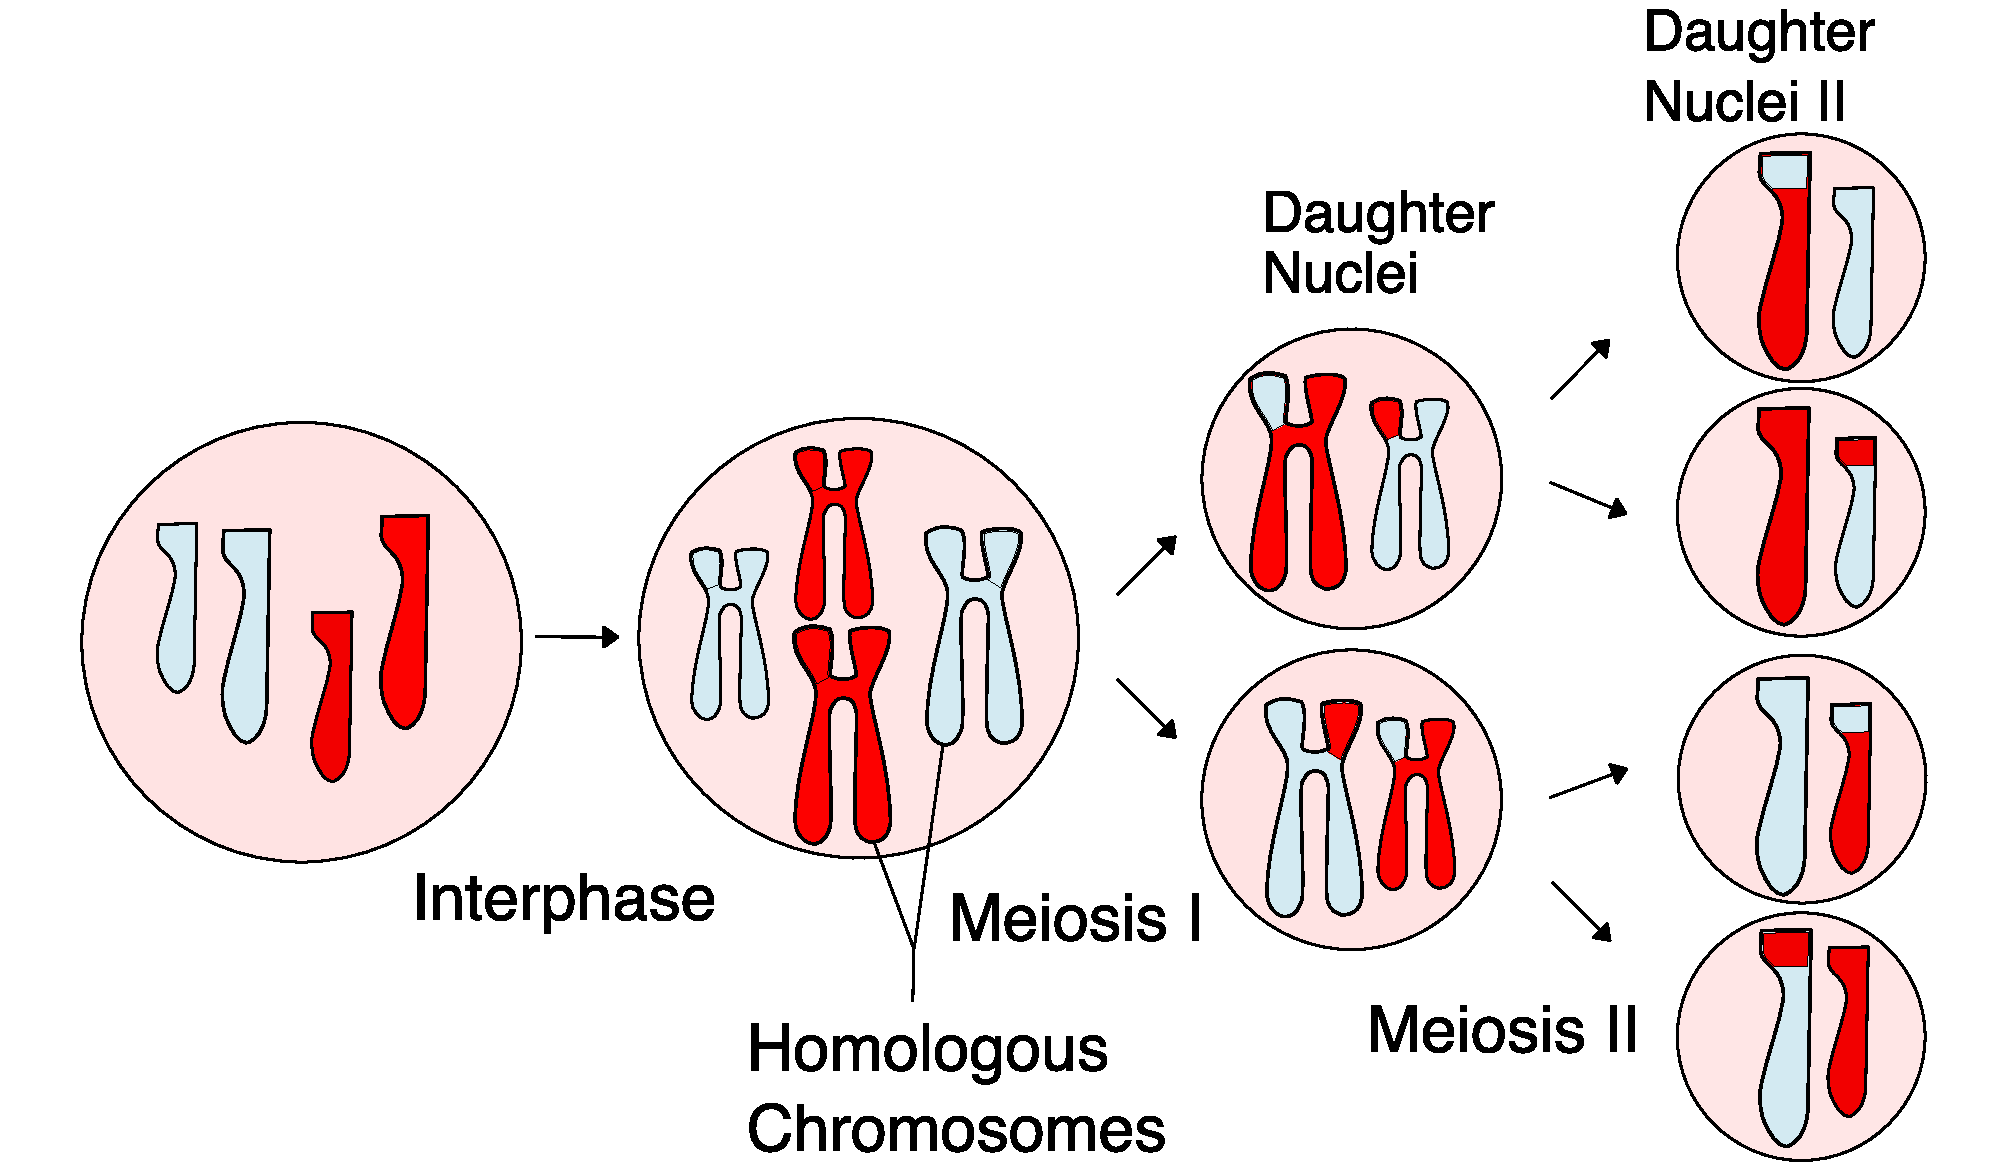
\includegraphics[width=0.8\linewidth]{meiosis}
    \caption{Overview of meiosis and an illustration of recombination between homologous chromosomes resulting in four unique daughter cells. Image reprinted from~\cite{} with permission.}
    \label{fig:meiosis}
\end{figure}

As in mitosis, each round of cell division can be divided in prophase, metaphase, anaphase, and telophase. We will elaborate Meiosis I in details, especially the Prophase I when the nuclear oscillation happens. 

$\bullet$ \emph{Prophase I}: prophase I is an important stage that many processes happened. Two of the examples are bouquet formation \cite{Wegener1980a} and homologous recombination \cite{Davis2001,Gerton2005}, both occurring in generic organisms. In the early state of Prophase, chromosomes are reorganized spatially, usually, the telomeres are clustered and attached to a small region of the nuclear membrane, forming a bouquet structure. This is called bouquet formation or telomere clustering in biology \cite{Chikashige1994,Wegener1980a,Niwa2000}, see in Fig \ref{fig:prophase} for an example in fission yeast. In the process of recombination, the homologous chromosomes, which are paternal and maternal pairs, align and exchange some parts of their DNA and usually results in the chromosomal crossover. Homologous recombination is critical for pairing and accurate segregation of the chromosomes in the later stage of Meiosis I. More interestingly, this stage is exact the period when the nuclear oscillation happens in fission yeast \cite{Ding1998,Wells2006}. We will devote this part to next subsection.

\begin{figure}[htpb]
    \centering
    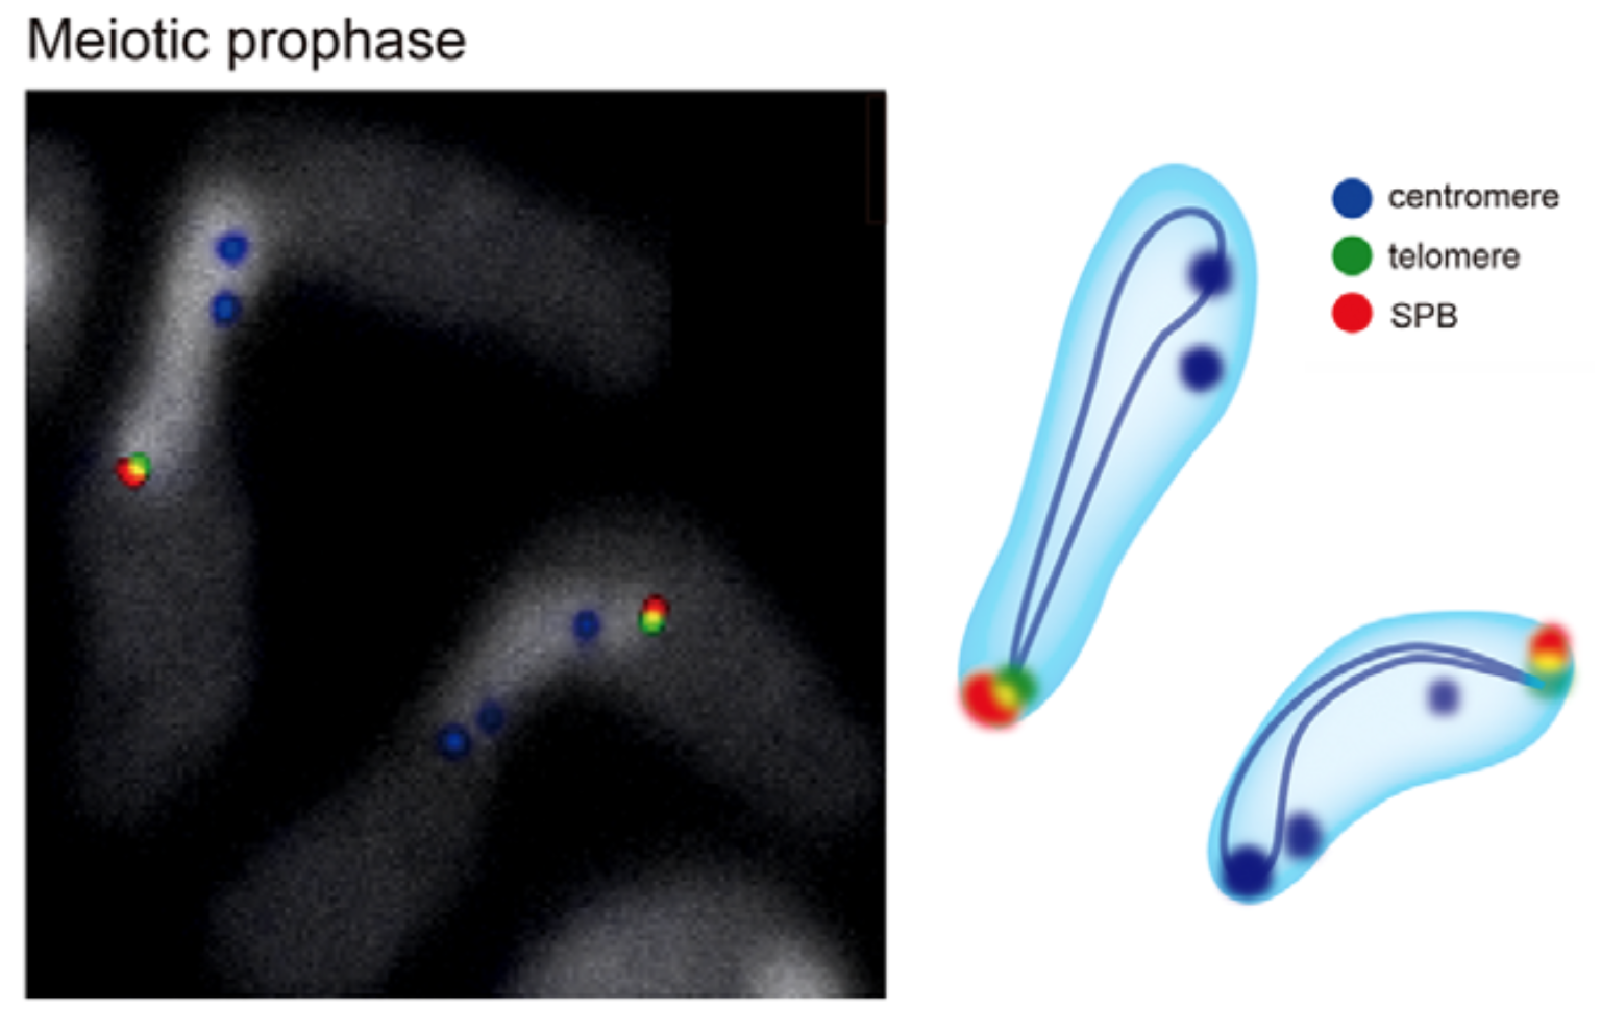
\includegraphics[width=0.8\linewidth]{prophase}
    \caption{The meiotic prophase I of fission yeast. Telomeres are clustered to form a bouquet structure. Image modified and reprinted from~\cite{Asakawa2007}.}
    \label{fig:prophase}
\end{figure}

$\bullet$ \emph{Metaphase I}: in this stage, homologous pairs move together along the middle plate, the microtubules from centrosomes attach to their respective chromosomes, the paired homologous chromosomes align along an equatorial plane that bisects the spindle. However, in Fission Yeast, the centromere is replaced by a functional equivalent organelle called spindle pole body (SPB)~\cite{Freeman2008}.

$\bullet$ \emph{Anaphase I}: in this stage, the microtubules shorten, pulling homologous chromosomes to opposite poles. Notice here, chromosomes still consist of a pair of sister chromatids. The cell body elongates, preparing for cell division~\cite{Freeman2008}.

$\bullet$ \emph{Telophase I}: in the last stage of Meiosis I, chromosomes arrive at the poles. The microtubules network of spindle disappears. New nuclear membrane appears. The two daughter cells now only have half the number of chromosomes~\cite{Freeman2008}.

After Meiosis I, Meiosis II occurs without DNA replication in between. The process is similar to Meiosis I except the sister chromatids segregate instead of homologous chromosomes~\cite{Freeman2008}. Four unique daughter cells are formed after the completion of Meiosis. The homologous recombination process takes an important role for this uniqueness.

\subsection{Nuclear oscillations}
\label{sub:nuclear_oscillations}

As mentioned in the previous subsection, nuclear oscillation happens during prophase I of meiosis in fission yeast, and so as the important processes of chromosomes homologous alignment and recombination~\cite{Ding1998}. Because the impressive shape of nucleus during this stage, nuclear oscillation also often mentioned as \emph{horse-tail} movements in biology\cite{Koszul2009a,Wells2006,Davis2001}, see in Fig.~\ref{fig:oscillation} for a time-lapse illustration. We believe the chromosome movements play an important role in this process and decide to model it quantitatively. In this subsection, we are going to elaborate the details of nuclear oscillation. We will answer the questions like what is the internal structure of nucleus during oscillation, what is the driven force of the oscillation, how long the oscillation lasts and what is the time period of the oscillation, etc.
\begin{figure}[htpb]
    \centering
    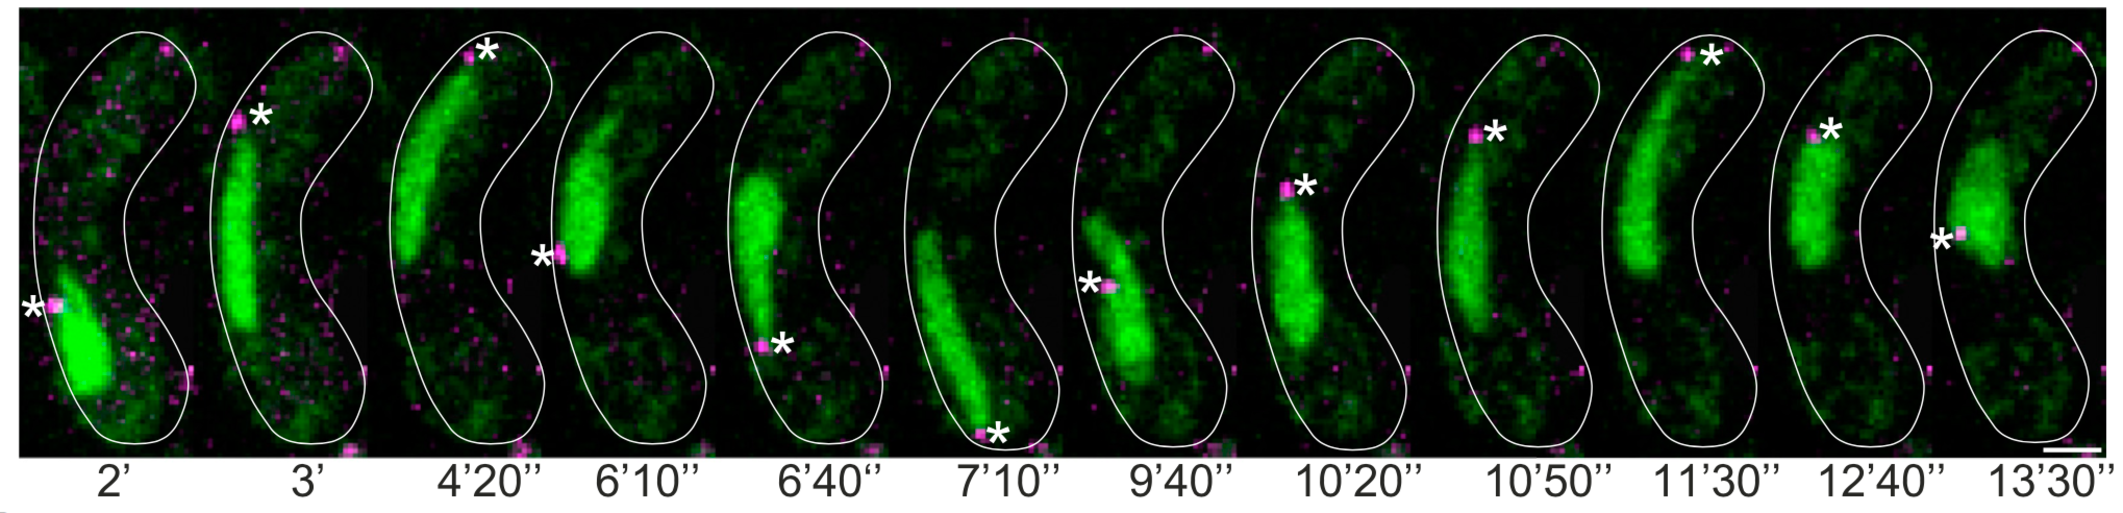
\includegraphics[width=1.0\linewidth]{oscillation}
    \caption{Time-lapse experiments of nuclear oscillation in fission yeast, DNA marker in green (Rec8-GFP) and SPB marker in magenta (Sid4-mCherry) also indicated by asterisk. Reprinted from~\cite{Chacon2016} with permission.}
    \label{fig:oscillation}
\end{figure}

\subsubsection{The looping structure of chromosomes}
Before the nuclear oscillation, chromosomes are reorganized and the bouquet formation happens. In fission yeast, the SPB is anchored in the nuclear envelope, telomeres of chromosomes are clustered to the SPB region of the inner nuclear membrane. The chromosomes are condensed to be the rod-like chain. Notice that there are still two sister chromatins contained in one chromosome. With all the telomeres bond to the SPB, chromosomes form the looping structure, as we can see in Fig.~\ref{fig:prophase}. 

\subsubsection{Redistribution of dynein motors drives the nuclear oscillation}
While the inner side of SPB bonds the chromosome telomeres, the outer side is attached to the microtubules in the cytoplasm. During the oscillation, dynein motors are the energy supplier. Interestingly, as one motor is not enough for the oscillation, the collective behavior of motors is observed to drive the nucleus motion. The spatial distribution of motor molecular varies during the oscillation. Motors accumulates in the side of fission yeast that the nucleus moves toward to. It is found that the pulling force is the main contribution that drives the oscillation~\cite{Vogel2009}.

\subsubsection{Related biological parameters of nuclear oscillation}
To study the dynamics during oscillation, several parameters are estimated experimentally and input into our model later. These parameters are summarized in table~\ref{tab:parameters}.

\begin{table}[htpb]
    \centering
    \caption{Parameters of fission yeast during meiosis}
    \label{tab:parameters}
    \begin{tabular}{l|l}
        \hline
        \textbf{Parameter} & \textbf{Value} \\
        \hline
        Typical size of nucleus          &  $3\mu$m \\
        Chromosome number                &  Three pairs \\
        Compaction ratio of chromatin    &  $10^2$bp/nm \\
        Kuhn length of chromatin         &  $100\sim300$nm  \\
        Duration of nuclear oscillation  &  $2$ hours  \\
        Period of nuclear oscillation    &  $10$ min  \\
        Moving speed of nucleus          &  $2.5\mu$m/min \\
        Viscosity of nucleoplasm         &  $1000\times \mu_{\text{water}}$ \\
        Length of Chromosome I           & $5.58$ Mb  \\
        Length of Chromosome II          & $4.54$ Mb  \\
        Length of Chromosome III         & $2.45$ Mb  \\
        \hline
    \end{tabular}
\end{table}


\subsection{The role of nuclear oscillations for chromosome alignment}
\label{sub:the_role_of_nuclear_oscillations_for_chromosome_alignment}


Although we can clearly observe the nuclear oscillation in fission yeast, the biological role of it is not thoroughly understood. One intuitive hypothesize is that the movement facilitates the paring of homologous~\cite{Ding2004}. However, Koszul et al. proposed that the chromosome movement might play other roles than paring, such as resolve homologous entanglements or non-homologous connections~\cite{Koszul2009a}. Also, Mariola et al. stated a dual role for the nuclear oscillation, promoting initial paring and restricting the time of chromosome associations to ensure proper segregation~\cite{Chacon2016}. 

We believe nuclear oscillation plays an important role for the chromosome alignment. However, it is hard to image the exact mechanism of the alignment without going deeper of the process. That is why we propose a quantitative model in this thesis and study the statistical and dynamical details of the model, trying to understand to the machinery of paring quantitatively. 


%********************************** %Second Section  *************************************
\section{Polymer model and DNA}
\label{sec:polymer_model_and_dna}
In this section, we will briefly introduce the theoretical models used to quantify the DNA. These models are characterized by beads connected by rods or springs, which embody the field of polymer physics. More specifically, we will mention the model we used for the chromosomal DNA during nuclear oscillation and summarize previous works of applying the polymer models to the chromosomal DNA. And the theoretical models about looped polymer and pulled polymer are discussed. Finally, we will discuss the conditions that allow us to use the equilibrium setting to study the intrinsic non-equilibrium polymer problems.  

\subsection{Models of chromosomal DNA}
\label{sub:models_of_chromosomal_dna}


To quantitatively describe the chromosome, it is natural to model it as a polymer model. In fact, there are already a lot of excellent examples in this direction~\cite{Wong2013,Tree2013,Halverson2014,Jun2010a}. However, depending on the situations under considering, different polymer models may applied. 

In physics, a polymer model is usually described by beads connected by massless springs or rods. The interactions, usually characterized as different types of potentials, specify the setting of the model~\cite{Doi1988}. As we want to model the chromosome during nuclear oscillation in fission yeast, there are two major factors we need to take into account besides some other minor details. First, the topology of the chromosome is a ring structure as shown in Fig.~\ref{fig:prophase}. Second, all chromosomes are bound to the SPB and pulled by an external force. According to these biological factors and the experimental measurements like Fig.~\ref{fig:prophase}, we propose a pulled polymer loop model for the chromosomes in this specific situation. See in Fig.~\ref{fig:schematic} for a sketch of our model. We will leave the discussion of the model details in afterward chapters.

\begin{figure}[htpb]
    \centering
    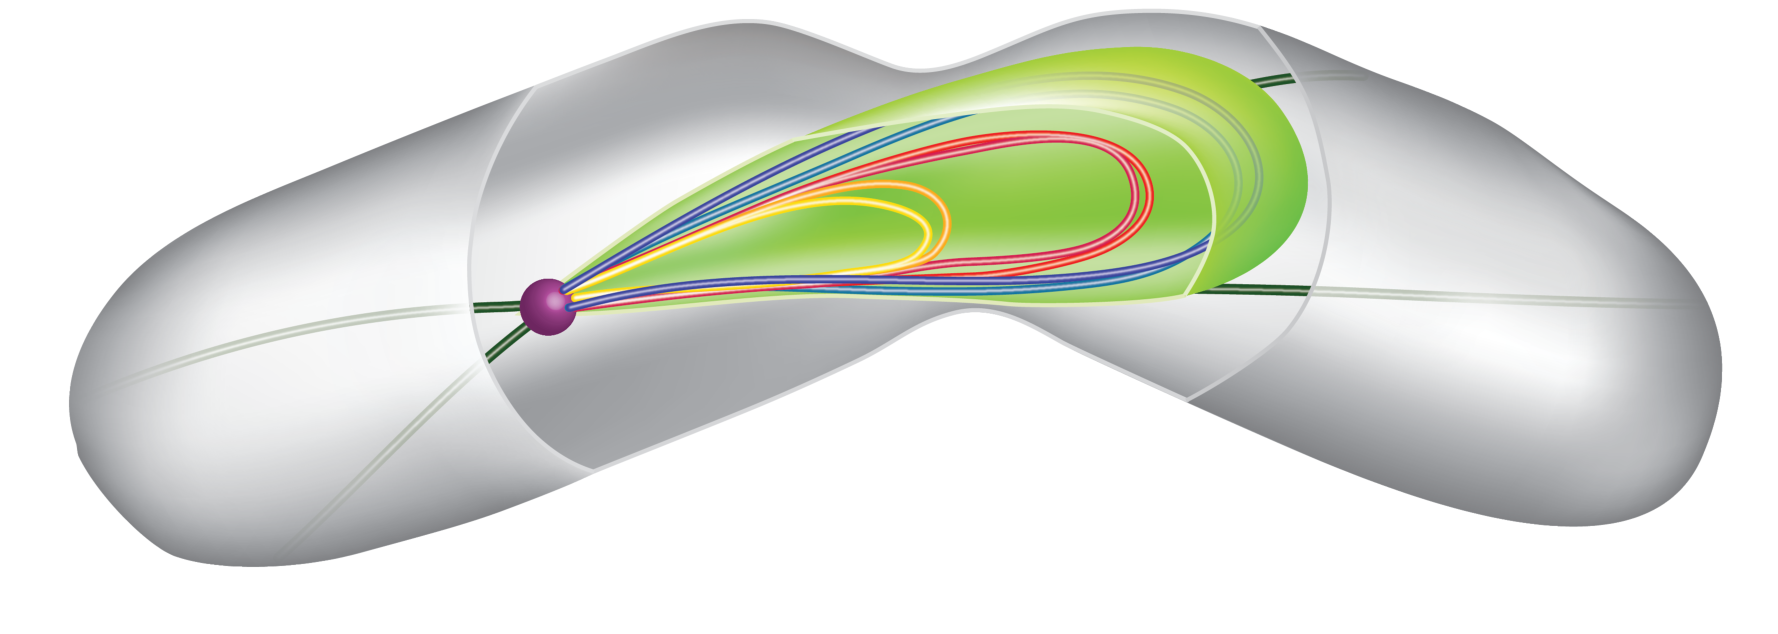
\includegraphics[width=0.8\linewidth]{schematic}
    \caption{The sketch of our pulled polymer loops model for chromosomes in meiotic fission yeast. Three pairs of chromosomes with all ends bound to SPB (shown in magenta) in the nucleus are indicated by different colors.  The SPB is pulled by multiple dynein motors (not shown) walking along microtubules (dark green). The SPB is anchored to the nuclear envelope (light green) and entrains the whole nucleus.}
    \label{fig:schematic}
\end{figure}

To the best of our knowledge, there are not many works which are discussing on not only the polymer loops but also the polymer is pulled by an external force. In the following subsections, we will introduce two related aspects of previous works, i.e. works about the polymer loops and works related to pulled polymer. 

\subsection{Polymer loop and pulled polymer model}
\label{sub:polymer_loop_and_pulled_polymer_model}

\subsubsection{Polymer loop model}
\label{ssub:Polymer_loop_model}

Polymers forming a looping structure are ubiquitous in chemistry and biology~\cite{Halverson2014,Richter2015}. The study of ring polymer can go back to the years when polymer physics was built up~\cite{Kramers1946,Zimm1949}. Kramers developed an equilibrium theory that possesses branch points and rings of the dilute polymer solution in 1946~\cite{Kramers1946}. Zimm calculated the statistics of mean square radii of molecules containing branches and rings in 1949~\cite{Zimm1949}. However, comparing to the simplest polymer chain model, research focus on polymer loop are far less than the former. We will review here some interesting and most related ones. Of course, it is not possible to exhaust all related works here, we pay our attention particularly to those that are related to the chromosome modeling.

Since Kramers and Zimm, there are a number of works trying to study the static and dynamical properties of the ring polymer from the theoretical point of view.
In 1965, Casassa derived some statistical properties of flexible ring polymers, including mean square radius, the second Virial coefficient and angular distribution of scattering~\cite{Casassa1965}. 1980, Burchard and Schmidt calculated the static and dynamical structure factors of flexible ring polymers~\cite{Burchard1980}. Baumg\"{a}rtner considered the self-avoiding effect of ring polymers in 1984 and found the asymptotic scaling exponents are the same as linear polymers \cite{Baumgartner1982a}. In 1986, Cates et al. studied the nor-concatenated ring polymer melt and found the size of polymer $R$ scales with the polymerization index $N$ as $R\sim N^{2/5}$ and the diffusion constant $D$ scales as $D\sim N^{-2}$ \cite{Cates1986}.  In 1994, Obukhov et al. considered the dynamics of a ring polymer in a gel and obtained the diffusion coefficient scales with the molecular weight as $D\sim M^{-2}$ and the longest relaxation time $T$ scales as $T\sim M^{5/2}$ \cite{Obukhov1994}. Carl investigated the configurational and rheological properties of multiple-twisted ring polymers using a long cyclic finitely extensible bead-spring model in 1995 \cite{Carl1995}. He also presented a study on bead-spring chains in steady flows, various properties such like the power spectrum, the autocorrelation functions of configurational quantities were discussed in 1996 \cite{Carl1996}.
In 2001, Panyukov and Rabin studied the effects of thermal fluctuations on elastic rings. Analytical expressions are derived for some static and dynamical quantities \cite{Panyukov2001}.  Mukherji et al. studied a polymer ring or chain diffused around attractive surfaces. They found the diffusion constant scales as $D \sim N^{-3/2}$ linear chain and solid strong adsorbed surfaces, and $D\sim N^{-1}$ for ring polymer and soft surfaces in 2008 \cite{Mukherji2008}. Sakaue proposed a simple mean-field theory for the structure of ring polymer melts which takes into account the many-body effects \cite{Sakaue2011,Sakaue2012}. In 2012, Kim et al. presented a self-consistent field theory formalism of topologically unconstrained ring polymers \cite{Kim2012}.  In 2013, Reigh performed lattice Monte-Carlo simulations to investigate the dependence of ring polymer conformation to the concentration, where the scaling of gyration radius with the concentration $R_g \sim \phi^{-0.59}$ was found \cite{Reigh2013}. In 2014, Lang et al. studied the tumbling dynamics of semiflexible ring polymers as a model of the cytoskeletal filament in a shear flow. They found the tumbling frequency scales $f_c$ scales with the Weissenberg number as $f_c \sim Wi^{3/4}$ rather than the prediction of classical theory that $f_c \sim Wi^{2/3}$ \cite{Lang2014b}.

Looped polymer with high concentration, like polymer melts, are often used in modeling interphase chromosomes. Interestingly, it is found that during interphase, the spatial organization for the multiple chromosomes in the nucleus is not homogeneous and well mixed. Instead, each chromosome forms its own ``territories'' \cite{Halverson2014}. Many interesting works can be found respecting to this problem. For example, in 2008, Rosa and Everaers used the simulation results of polymers to explain the existence and stability of territories of interphase chromosomes in genetic eukaryotes \cite{Rosa2008}. Because usually, the computation power required to simulate the whole genome is huge, they also developed an efficient multiscale numerical approach to study the conformational statistics of ring polymers melts in \cite{Rosa2014b}.  Dorier employed a very simple non-permeable freely jointed polymer model and recovered the chromosomal territories in a crowded nuclei \cite{Dorier2009}. This part of work is well reviewed in \cite{Halverson2014}, the interested reader can refer to the references therein. 

On the other hand, it is also possible that looping structures of polymer are formed temporarily in chromosomes. This could be caused by the DNA replication process or binding proteins connecting two loci of chromosomes. Many great works were done also in this direction. In 1995, Sachs use a looping random walk model to study to the interphase chromosomes, fluorescence labeled data is compared to the theoretical prediction \cite{Sachs1995}. Marko considered a model of two polymer loops tethered one another and its application to chromosome segregation in 2009 \cite{Marko2009}.  The looping probabilities of interphase chromosomes were also discussed in \cite{Rosa2010}.  In 2011, Zhang et al. modeled the meiotic chromosomes as a polymer that could form internal loops by binding proteins. They found the loops play an important role in the mechanical properties of the polymer \cite{Zhang2011a}. Wong set up a polymer model and use it to predict the whole nuclear architecture of fission yeast \cite{Wong2012}. Dekker and Giorgetti employed the computational polymer model to explain the 3C/HiC data \cite{Dekker2013,Giorgetti2014}. In 2014, Youngren employed ring polymer model to study the duplication and segregation of \emph{E. coli} chromosomes \cite{Youngren2014}.  These are just a few examples, more can be found if one is interested.

The confinement such as the nuclear membrane or cell shape could also take an important role in chromosome dynamics. One of the examples of this kind of work is Fritsche's work in 2011, they studied the influence of confinement geometry to the spatial organization of semiflexible ring polymers \cite{Fritsche2011}. The studies of the polymers (including chains and rings) under confinements were reviewed by Ha el al. in \cite{Ha2015}. 

There are also a lot of great experimental work related to polymer loops. In 1992, Tead et al. employed polystyrene molecules to perform experiments and compared the diffusion of linear and ring polymers \cite{Tead1992}. Kapnistos et al. found the stress relaxation of entangled ring polymer was power-law rather than exponential in \cite{Kapnistos2008}. Structure and dynamics of polymer loops by neutron scattering were studied by Br\'{a}s et al. in 2011. Witz et al. employed the atomic force microscopy to studied 2D circular DNA in \cite{Witz2008,Witz2011}.  Goo{\ss}en et al. studied dynamics of polymer loops using neutron spin echo spectroscopy which space-time evolution of segmental motion could be observed \cite{goossen2014,Goossen2015}. 

Due to its importance, the study of polymer loops is much intensive and causes much more attention nowadays. Besides what we have mentioned above, the shape of ring polymers is studied in \cite{Bishop1985,Jagodzinski1992,Alim2007,Reiss2011}. Also, there are a series of works considering the ring polymer with entanglements and topological knots \cite{Michels1982,Polymers1991,Koniaris1991,Grosberg1996,Shimamura2001,Orlandini2003,Tubiana2011,Uehara2014,Li2015a}.
We are only able to list a few of those great works. Interested readers can refer to the references therein. 

\subsubsection{Pulled polymer model}
\label{ssub:Pulled polymer model}

As we mentioned above, in order to model the nuclear oscillation of fission yeast, we have to consider the pulling dynamics. If we transfer the coordinate and sit on the pulled monomer, a pulled polymer is also equivalent to a pinned polymer in an external flow or force field. In this section, we would like to review some previous works in this direction. Most of them are about pulled polymer chain. Whatsoever, we think it is still helpful to know what have been done about pulled polymers or tethered polymer in an external field.

A polymer chain with one end free and the other end pulled by an external force was first discussed by de Gennes \cite{DeGennes1974,DeGennes1979}. After that, another important progress was made by Pincus, he developed what is now called Pincus theory \cite{Pincus1976,Pincus1977}, which consider the pulled polymer as a sequence of independent ``blobs''.  Brochard-Wyart further developed the ``trumpet'' and the ``stem-flower'' pictures of pulled polymer chain \cite{Brochard-Wyart1993a,Brochard-Wyart1994a,Brochard-Wyart1995,Adjarei1995a}. When the pulling force is not too strong, the polymer presents as a series of independent blobs with increasing size, i.e. the portion of polymer near to the free end fluctuates more. As the pulling force increased to a strong regime, the polymer portion near to fixed end is totally stretched, forming a ``stem-flower'' like picture, see in Fig. \ref{fig:stemFlower}.  
Using fluorescence microscope and optical tweezers,  Perkins et al. performed the pulling experiments on single DNA molecule and found the results consistent with the Brochard-Wyart's theory \cite{Perkins1995a,Perkins1994}. They also measured the relaxation time of this pulled polymer and obtained the scaling $\tau \sim L^{1.66}$ \cite{Perkins1994a}. Wirtz also confirmed the theory by measuring transport properties of a single DNA molecule in \cite{Wirtz1995}.

\begin{figure}[htpb]
    \centering
    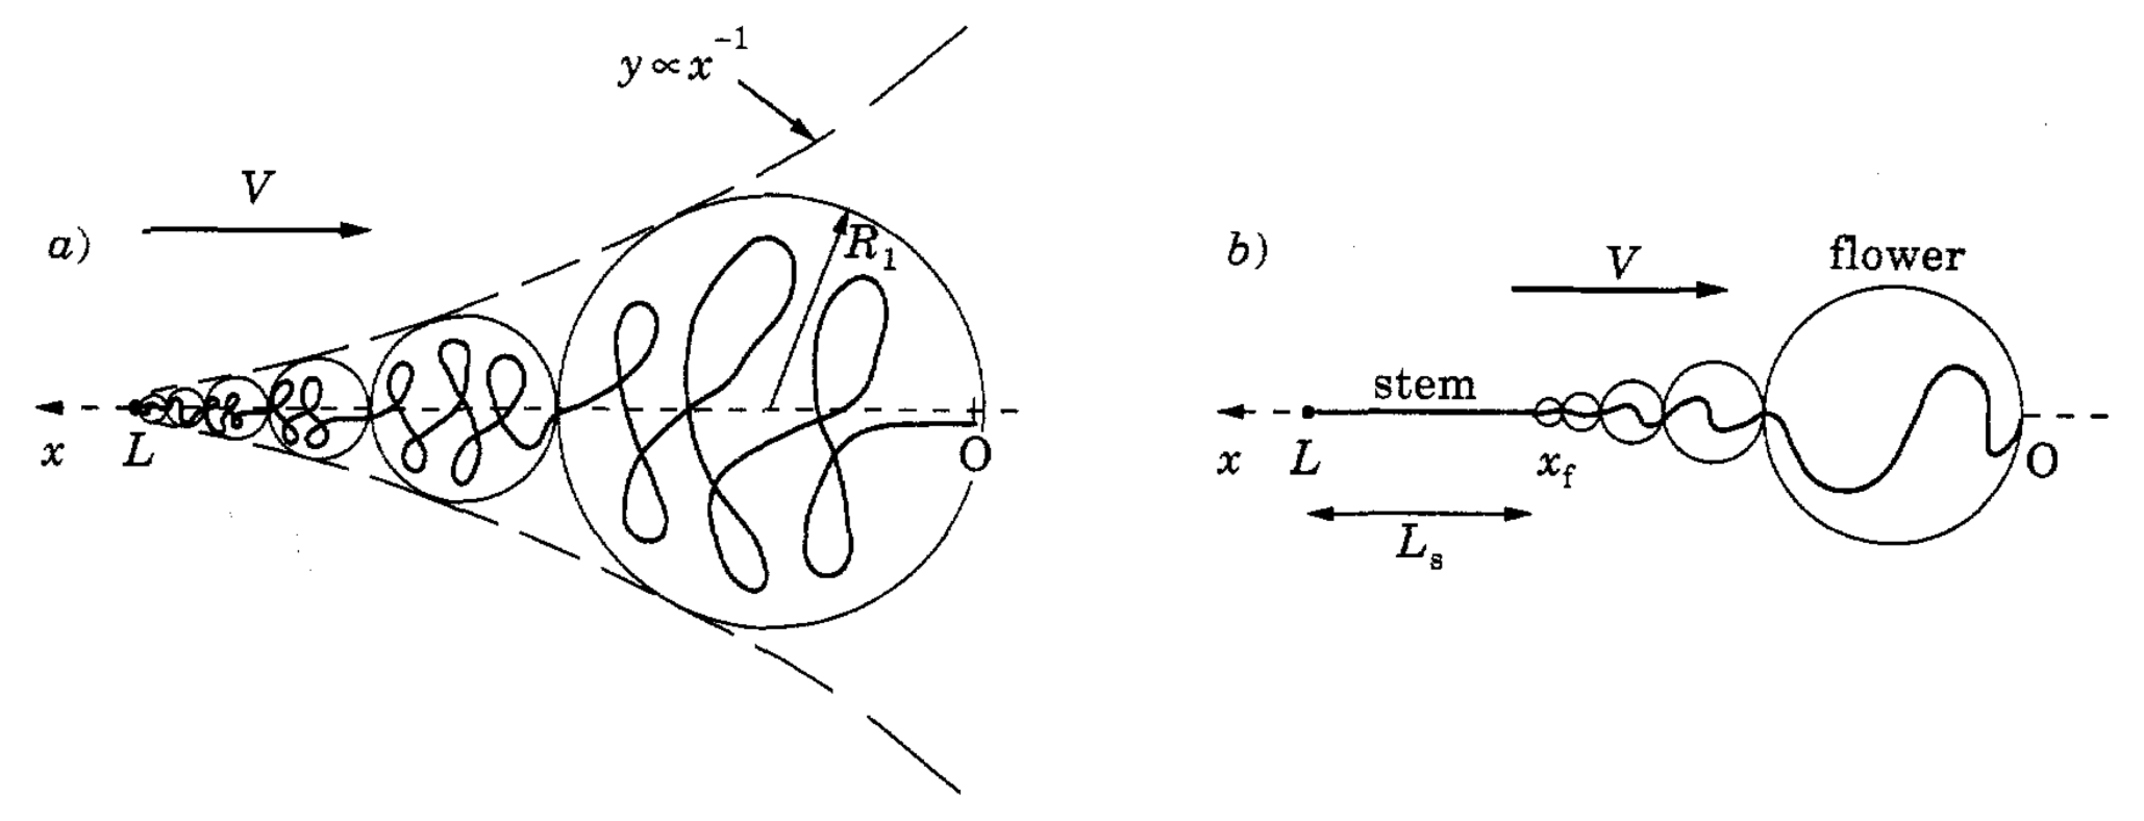
\includegraphics[width=0.8\linewidth]{stemFlower}
    \caption{Illustration of ``stem-flower'' picture for pulled polymer chain. (a) Trumpet picture at moderate pulling force; (b) Stem-flower picture at strong pulling force. Image reprinted from \cite{Brochard-Wyart1995}.}
    \label{fig:stemFlower}
\end{figure}


Rezehak et al. considered pinned polymer in a uniform flow with hydrodynamic interaction and proposed a so-called f-shell blob model \cite{Rzehak1999}. Larson et al. performed Brownian Dynamics simulation for a DNA in an external flow field \cite{Larson1999}. In 2000, Doyle measured the cyclic and stretching dynamics of a tethered DNA molecule in the shear flow \cite{Doyle2000, Ladoux2000a}. Sebastian studied the dynamics of pulling a polymer out of a potential well \cite{Sebastian2000}. Cui performed the stretching and releasing experiment by pulling a single chicken erythrocyte chromatin fiber with the optical tweezers \cite{Cui2000a}. Rzehak discussed the conformation fluctuation and relaxation of a tethered polymer in uniform flow \cite{Rzehak2003a}. In 2007, Mohan et al. employed Rouse theory to study the unraveling dynamics of tethered semiflexible polymer in uniform solvent flow \cite{Mohan2007}. Sing et al. studied flexible and semiflexible tethered polymers in the limit of high shear flows and consequently near-full extension of the chains in \cite{Sing2011}.  Sakaue et al. studied the conformation and dynamics of a single flexible polymer chain that is pulled by a constant force applied at its one end, finite extensibility, the excluded volume, and the hydrodynamic interactions are discussed \cite{Sakaue2012a}.  Varghese et al. investigated the force fluctuations in stretching a tethered polymer \cite{Varghese2013}.
In 2013, Dai and Doyle found in \cite{Dai2013a} that the scenario of a pulled polymer is very similar to a polymer confined in a cylinder with proper radius.

To the best of our knowledge, the discussion of pulled polymer loop is missing except our own work \cite{Lin2015}. So we reviewed here the works about polymer loop on one side and the works of pulled polymer on the other side. Of course, the details are not shown here, interested readers can go into the references.

\subsection{Equilibrium vs non-equilibrium}
\label{sub:equilibrium_vs_non_equilibrium}

Usually, the problem related to polymers in the solution are intrinsically non-equilibrium due to the highly fluctuating environment. However, it is possible to treat it as an equilibrium if certain conditions are satisfied.
The important thing is about the characteristic length and time scales. Here, let us discuss this topic in the circumstance of nuclear oscillation in fission yeast. 
\begin{figure}[htpb]
    \centering
    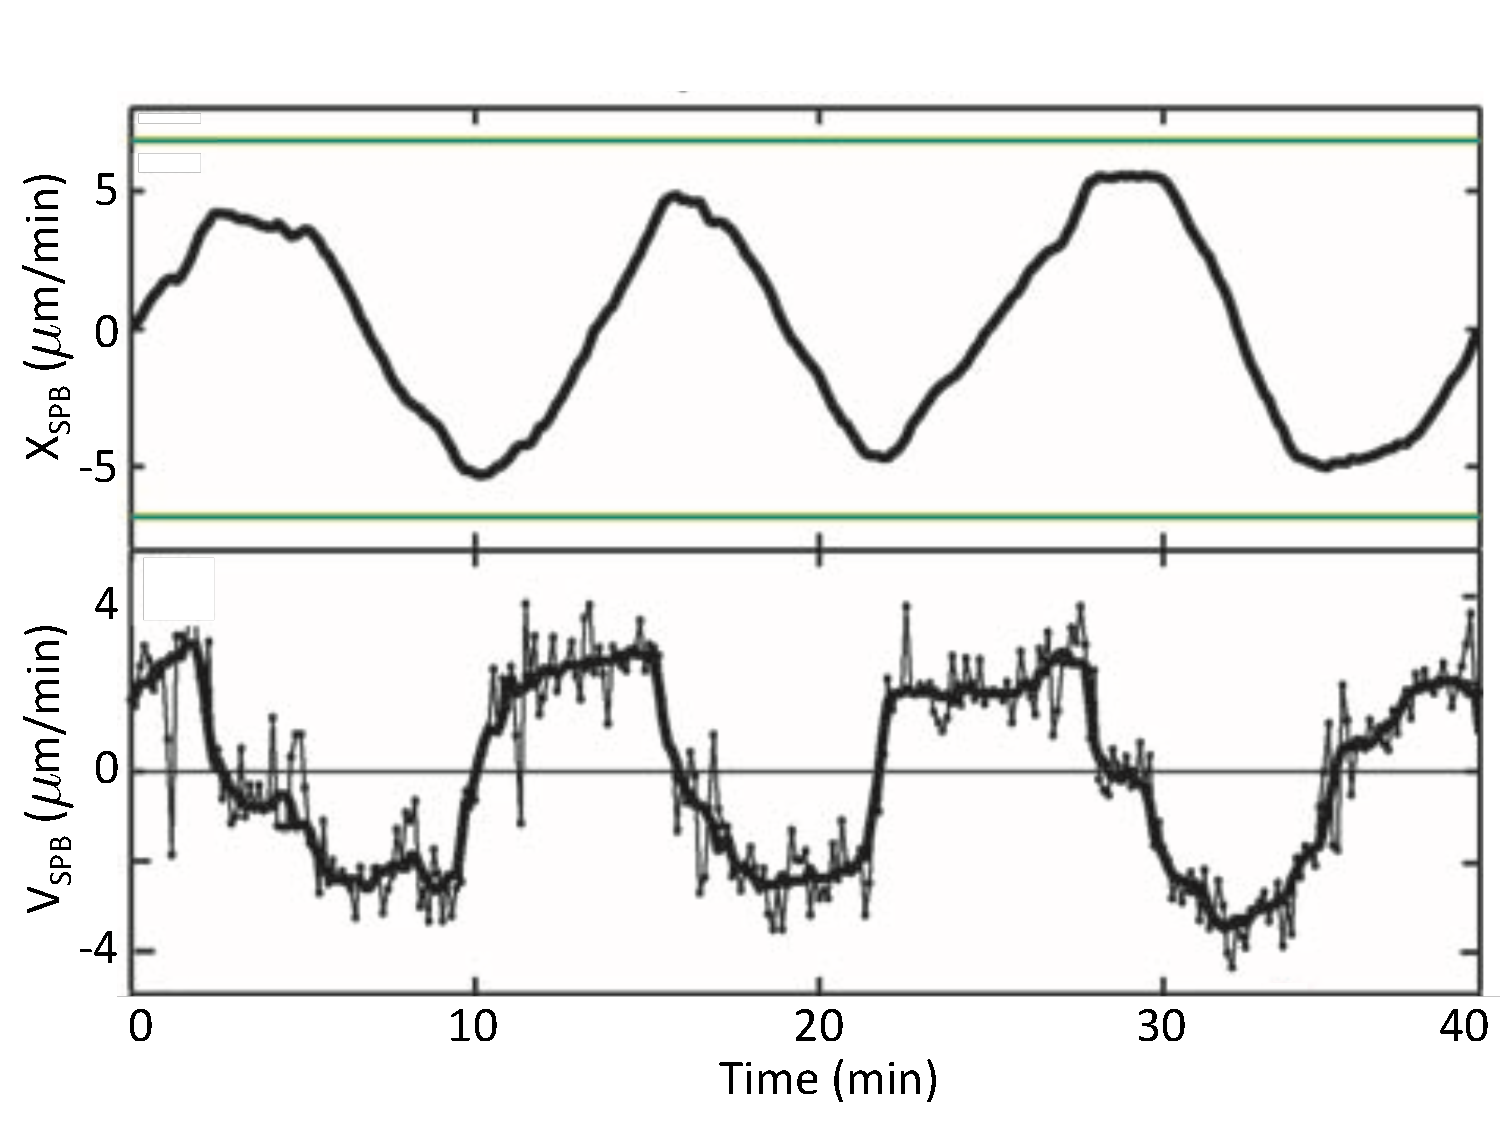
\includegraphics[width=0.8\linewidth]{vspb}
    \caption{Experimental trajectory and velocity of the SPB measured by florescence microscopy. The upper panel shows the trajectory of the SPB along the cell main axis. Green line is the boundary of the cell. The lower panel shows the corresponding velocity of the SPB. Image reprinted and modified from \cite{Vogel2009}.}
    \label{fig:vspb}
\end{figure}

The size of the fission yeast is about $10$ microns. Once we model the chromosomes polymer model of bead-rod or bead-spring, the size of monomer bead can be estimated to be $30-100$ nm \cite{Vogel2009, Chacon2016}. In this length scale, the thermal fluctuation is important. The thermal fluctuation is determined by a characteristic temperature, which depends not only on the room temperature of the environment, but also some stochastic collisions between molecules in the nucleus. Here we will assume the level of fluctuation is stable, which means the characteristic temperature is a constant. This is one of the essential conditions to allow us consider the polymer problem as an equilibrium problem.

On the other hand, the nuclear oscillation in fission yeast is an oscillating dynamics. So in principle, the system is out of equilibrium by definition. However, notice that the time period of the nuclear oscillation is about $10$ mins. The oscillation can be divided into two parts. The chromosomes move towards to the opposite direction in each part. Moreover, experimental evidence shows that the velocity of the SPB is almost constant when moving towards one direction. See in Fg. \ref{fig:vspb}. 
If the relaxation time of the system is much smaller than half of the oscillation period, then it is proper to think the system as a equilibrium system. Actually, we will show in chapter 4 that this is indeed true under the setting of pulled polymer loops. It turns out the relaxation time scale is $\sim10$ s. As the characteristic time scale is much smaller than the oscillation period, so it is appropriate to consider the equilibrium statistics of the polymers when moving towards on direction. 

In fact, we will model the chromosomes as pinned polymer loops in an constant external force field. The equilibrium statistics will be discussed in chapter 3. 

In this section, we introduced the models we will use for the chromosomes of fission yeast chromosomes. We discussed what has been done for polymer models of DNA, especially the looped polymer and pulled polymer. Also, the conditions under which our polymer model can be considered as an equilibrium problem were discussed. In next section, we will discuss the other model which will be used in this thesis, which is ASEP.

%********************************** %Third Section  *************************************
\section{ASEP and Bethe ansatz}
\label{sec:asep_and_bethe_ansatz}
ASEP stands for Asymmetric Simple Exclusion Process. It is a 1D lattice model with many particles hopping on the lattice. The number of particles sitting on one lattice cannot be larger than one, which means the particle are exclusive to each other. Normally, the hopping rate of particle to right and left are not the same, which accounts for the asymmetric. It is one of the simplest model for system out of equilibrium. In this thesis, we found a very peculiar mapping from the polymer dynamics to the ASEP model. With the mapping, sophisticated methods and tools such as Bethe ansatz can be used to solve our problem. In this section, we will briefly introduce the history of the ASEP model and the Bethe ansatz method we used to find the exact solution of the model. 

\subsection{Brief introduction of ASEP}
\label{sub:brief_introduction_of_asep}

ASEP model is said to be a minimal non-equilibrium model similar to the Ising model in equilibrium statistical physics \cite{Derrida1998, Mallick2011b}. Interestingly, it is first proposed for the study of a biological problem. In 1968, MacDonald et al. proposed a mathematical model for the kinetics of protein synthesis by ribosomes, which is essentially the ASEP model \cite{Macdonald1968}. However, the name of ASEP is introduced later in 1970 by Spitzer with the aim of rigorously derive macroscopic hydrodynamic behavior from a microscopic model \cite{Spitzer1970}. The task is done by Varadhan et al. on this specific simple model \cite{hsu1999}. ASEP model has a lot of applications besides those mentioned above. Other examples ranging from the motion of motor molecules along the micro-tubes to the traffic systems \cite{Bressloff2013, schadschneider2010}. 

\begin{figure}[htpb]
    \centering
    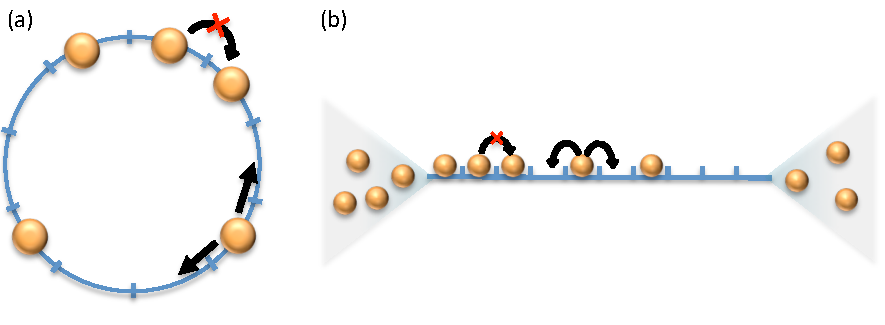
\includegraphics[width=1.0\linewidth]{asepSchematic}
    \caption{Schematics of ASEP model. (a) ASEP with periodic condition. (b) ASEP with open boundary condition.}
    \label{fig:asepSchematic}
\end{figure}

The simplest ASEP model is ASEP with periodic boundaries \cite{Mallick2011b}. See a schematic in Fig. \ref{fig:asepSchematic} (a). The stationary measure is simply a uniform distribution. If the hopping rate is asymmetric, then a steady current will be induced in the stationary measure. This is one of the simplest example that detailed balance is not satisfied in the stationary state. The full dynamics of this case can be solved by the Bethe-ansatz method \cite{Batchelor2007}, we will discuss more about the method later. 

People are also interested in the case of ASEP on a infinite line from theoretical point of view \cite{Levitt1973,Barkai2010a,Chou2011}. For example, one can derive rigorously the diffusion behavior of a tagged particle for the special case of symmetric hopping rate. 
\begin{equation}
    \label{eq:diffusionInfASEP}
    \left< x^2 \right> = 2 \frac{1-\rho}{\rho}\sqrt{\frac{t}{\pi}},
\end{equation}
where $\rho$ is the density of particles. So we can see it is a sub-diffusion process as long as $\rho\neq 0$. This phenomenon is observed in the experiments \cite{Chou2011}.

ASEP with open boundaries is consider as the minimal microscopic model of transport \cite{Crampe2014b, Mallick2011b}. See in Fig. \ref{fig:asepSchematic} (b). In this model, the two ends of the lattice is connected to two different reservoirs. So the rate of insertion and removal are different at the two ends. For instance, in the simplest case, particles can only be inserted at one end and removed at the other end, which is called totally asymmetric (TASEP). A current can be induced by the bias of hopping rates. In 1991, Krug et al. studied the ASEP with open boundaries and discovered the boundary induced phase transitions in the model. Depending on the insertion or removal rates at the ends, the stationary state of the system can be in high density, low density or maximum current phase. And the phase transition can occur by adjusting those boundary conditions \cite{Krug1991}. 

In order to solve the stationary state of the open ASEP, Derrida et al. proposed an approach which is now called Matrix Product Ansatz. It is a brilliant method far more useful than it was though to be at the beginning. Interested readers can refer to the excellent review paper for more details \cite{Derrida1998}. There is a booming of researches on the topic of ASEP after the work of Derrida and his co-workers. A lot of people make significant contributions to the field. For example, De Gier found the exact solution of open ASEP with certain special constraints in 2005 \cite{DeGier2005}. Spohn et al. constructed an exact solution of the KPZ equation using the ASEP in 2010 \cite{Sasamoto2010}. 

Despite the simplicity of the ASEP model, the way to find the solution of general open ASEP system is still an open question \cite{Crampe2014b, Mallick2011b}. There are a lot of efforts working in this direction. Although the Matrix Product Ansatz is widely used in the study of the stationary state ASEP. The Bethe-ansatz method is more powerful when it comes to the dynamics. 

Besides the periodic ASEP and open ASEP, the ASEP model we will discuss in details is the ASEP with reflecting boundaries. There are not so many works on this case. One of the exceptions are the work of Sch\"{u}tz et al. in 1994. They investigated the reflecting ASEP using the $U_q(SU(2))$ quantum group \cite{Sandow1994}. The exact stationary solution was found but not the dynamics. The reason for the lack of study on this specific case might be the inanimate steady state. There is no current in the stationary state, which makes the system looks boring. However, we will show that it is actually quite interesting especially when we notice the mapping from ASEP to polymer dynamics.

We will solve the reflecting ASEP completely using the Bethe ansatz method. So let us introduce briefly about the Bethe ansatz method here.
% We will discuss more about it because we are going to use a generated version of this method to solve the reflecting ASEP in our problem. However, before go into the detailed calculations, let us first discuss some interesting numerical results, which also works as the hints for the searching of the exact solution.

\subsection{Bethe ansatz}
\label{sub:bethe_ansatz}

Bethe-ansatz is a method proposed by Hans Bethe in 1931 in order to solve the Heisenberg spin chain model with periodic condition \cite{Bethe1931}. At that time, he did not realize his great work opened a new branch of physics which is now called the integrability theory \cite{Batchelor2007}. In 1963, Lieb-Liniger use the Bethe-ansatz method solved the Bose gas with $\delta$ interaction potential \cite{Lieb1963a,Lieb1963}. 

Another important application of Bethe-ansatz is the six vertex model which is also solved by Lieb. The next big step was the discovery of the Yang-Baxter equation, which is introduced independently by C.N. Yang and Rodney Baxter \cite{Yang1967,Baxter1972}. The Yang-Baxter equation provides a criteria to find out whether a model is integrable model or not \cite{Batchelor2007}. The investigation of the Yang-Baxter equation led to the introduction of quantum group theory and the theory of topological knot invariants etc. 

During 1970s and 1980s, advanced Bethe-ansatz methods like functional Bethe-ansatz  and algebraic Bethe-ansatz were developed \cite{Mallick2011b}. After the introduction of the ASEP model, these Bethe-ansatz methods were quickly adopted to find solution of these many particle system because of the intrinsic connection from ASEP to a spin chain system. For example, the solution of periodic ASEP is almost identical to the Heisenberg spin chain with periodic condition \cite{Mallick2011b}. The study of ASEP and Bethe-ansatz is still a very active field. There are a lot of references one can refer to \cite{Derrida1998,Liggett1999,Schutz2001,Golinelli2006,Mallick2011b}. 

In this section, we briefly introduced the ASEP model and the Bethe ansatz method. In next section, we will list the research goals of this thesis and the overview of this thesis.


%********************************** %Fourth Section  *************************************
\section{Outline}  %Section - 1.4
\label{sec:outline}
With the introduction of the biological problem and the background of polymer modeling as well as ASEP in previous sections, we are ready to go into the details of our study. In this section, we will propose our research goals for this thesis and give an overview for the organisation of the thesis.  

\subsection{Research goals}
\label{sub:research_goal}

The research goals of this thesis are listed as following:

$\bullet$ Propose a polymer model to describe the chromosomes in fission yeast during nuclear oscillation. The model is actually already mentioned in the previous section, i.e. the pulled polymer loop model. However, the details of the model will be discussed in the following chapters.

$\bullet$ Develop the quantitative theory for our pulled looping polymer model. As far as we know, there is no previous work on this issue. On the other hand, it is shown by the experimental facts lead us to a model with such settings.

$\bullet$ Perform numerical simulations of for the polymer model. The theory about an idealized model are always needed for numerical verifications. On the other hand, it is possible for the simulations to take into account of some complex biological factors in order to justify the assumptions of our theoretical model.

$\bullet$ Using the physical insights to understand to biological processes such as chromosome alignment. Understand the biology is our ultimate goal. The chromosome movements during cell division are so important that many diseases are related to that, such as Down syndrome \cite{Patterson2009}. Our understanding from physical layer helps to fight with these diseases.

In short, we want to quantitatively model the chromosome dynamics during the nuclear oscillation and use it to understand the biology. 

\subsection{Overview of the thesis}
\label{sub:overview_of_the_thesis}

The nuclear oscillation in fission yeast has been studied intensively from biological point of view. As far as we known, the quantitative modeling of chromosome dynamics is still missing. In thesis thesis, we propose an pulled polymer loop model to discuss the movements of meiotic chromosomes in fission yeast. More specifically, the chromosomes moving in one direction is modeled by polymers in a constant force field. We found a peculiar mapping from polymers to the particles on lattice. Using the mapping the equilibrium statistics of and relaxation dynamics are solved analytically. Furthermore, extensive simulations were performed to verify our theory and compare to the experimental data.

In chapter 2, we discuss the details of our pulled polymer loop model. Two realization of the model, i.e. bead-rod model and bead-spring model are introduced. We introduce a coordinate transformation so that the pulled polymer loop is transferred to the pinned polymer loop in an external force field. We then discuss the simulation techniques of the polymer model, including the Brownian Dynamics simulation and the Monte-Carlo simulation specific for the bead-rod model. 

In chapter 3, we solve the equilibrium statistics of pinned polymer loop in an constant external force field. The system is solved firstly in 1D by several different methods. The mapping from polymer loop to a particle system on lattice sites is illustrated. Then we extend our solution to the three dimensional setting. The mean and variance of each bead position are calculated. Moreover, we also discuss the case that a pair of polymer loops which represents homologous in the biological context. And the case of two intersecting loops represents one more connection of homologous through the centromeres is calculated. Based on the solution of equilibrium statistics, we also quantify the shape of the pinned polymer loops in the external force field. 

In chapter 4, we investigate the relaxation dynamics of the pinned polymer loop in an external force field. First, we try to apply the Rouse theory on the pinned polymer loop model. However, we find the Rouse theory does not work because the unrealistic result which shows the relaxation time of the polymer is independent of the strength of the external force field. We then illustrate the peculiar mapping from polymer dynamics to the particle hopping of ASEP. The pinned polymer loop model is mapped to reflecting ASEP system with exactly half of the lattice sites occupied. And then the Bethe ansatz method is employed to find the exact solution of the ASEP system. Results from ASEP are mapped back to the polymer loop model to discuss the relaxation dynamics of polymer. And the 3D simulations are performed to verify the theory. The dynamics of stretch and coil transition is discussed briefly.

In the last chapter, chapter 5, we first summarize our results by a discussion on applying the theory to the real fission yeast context. And the stationary shape of pinned polymer loops derived from our theory is compared with the previous blob theory, which is about the ``stem-flower'' picture of pinned polymer chain. On the other hand, the relaxation time from our theory is compared the known experimental results on optical trapped $\lambda$-DNA. Finally, we give an outlook of this thesis in the last section.







